%           %experimenting with svn-multi

\svnkwsave{$RepoFile: siminos/froehlich/flow.tex $}
\svnidlong {$HeadURL$}
{$LastChangedDate$}
{$LastChangedRevision$} {$LastChangedBy$}
\svnid{$Id$}


\chapter{\CLf}
\label{chap:blog}

     \Private{
\noindent{\bf Rebecca -
Jun 16 - Aug 21 2009}:\\
     }
This project first reproduces results reported by
Siminos\rf{SiminosThesis}, and then investigates various ways
of `quotienting' the \SOn{2} symmetry of \cLe, and reducing
the dynamics to symmetry 4-dimensional \reducedsp.
     \PC{
   When you write
   a project report or a research article, you always write abstract, introduction
   and conclusions first, and then keep rewriting them often.
   They are the most important parts of the text, as that is
   for most people only parts they will look at.
   }


The project consists of my notes and exercises. The flow of
the argument is in the classical
\HREF{http://en.wikipedia.org/wiki/Socratic_method}{Socratic dialogue}
mode; question, answer, question, $\cdots$.
    %
    \Private{ % subversion label pages
$\footnotemark\footnotetext{{\tt \svnkw{RepoFile}}, rev. \svnfilerev:
 last edit by \svnFullAuthor{\svnfileauthor},
 \svnfilemonth/\svnfileday/\svnfileyear}$
    } % end \Private{

The \cLe\ were introduced by Gibbon and McGuinness\rf{GibMcCLE82}
as a low-dimensional model of baroclinic instability in the
atmosphere. In the complex form, they are given by
\beq
\begin{split}
 \dot{x} &=-\sigma x+ \sigma y \\
 \dot{y} &=(r-z)x-a y \\
 \dot{z} &= \frac{1}{2}(x y^*+x^*y)-b z\,
 \label{eq:CLe}
\end{split}
\eeq
where $x,y$, $r=r_1+ i\,r_2$, $a=1+i\,e$ are complex and $z$,
$b$, $\sigma$ are real. Rewritten in terms of real variables
$x=x_1+ i\, x_2\,,\ y=y_1+i\, y_2$, \cLe\ are a 5-dimensional
first order ODE system\rf{SiminosThesis}
\beq
\begin{split}
	\dot{x}_1 &= -\sigma x_1 + \sigma y_1\\
	\dot{x}_2 &= -\sigma x_2 + \sigma y_2\\
	\dot{y}_1 &= (r_1-z) x_1 - r_2 x_2 -y_1-e y_2 \\
	\dot{y}_2 &= r_2 x_1 + (r_1-z) x_2 + e y_1- y_2\\
	\dot{z} &= -b z + x_1 y_1 + x_2 y_2\,.
	\label{eq:CLeR}
\end{split}
\eeq
In all numerical calculations that follow we shall set the
parameters to the Siminos values\rf{SiminosThesis},
\beq
r_1=28,\; b=\frac{8}{3},\;
\sigma=10,\; e=\frac{1}{10},\quad \mbox{and} \quad r_2=0
\,.
\ee{SiminosPrmts}

Here we are not interested in the physical applications of
these equations; rather, we study them as a simple example of
a dynamical system with continuous (but no discrete)
symmetries. Our goal is to find computationally
straightforward method of reducing the dynamics to a
lower-dimensional \statesp, where each group orbit of the
full system (\ie, set of translationally equivalent states)
is represented by a single point. If successful, the methods
that we develop might be applicable to very high-dimensional
flows, such as translationally equivariant fluid flows
bounded by pipes or planes\rf{GHCW07,GibsonMovies}.

\noindent {\bf Acknowledgments.}
This report is written in collaboration with
E.~Siminos and P.~Cvitanovi\'c.
S.F. work was supported by the National Science Foundation
grant DMR~0820054.
P.C. thanks Glen Robinson Jr. for support.

\subsection{Visualizing \cLf}

In \refexer{exer:PlotCLf} we simulate \cLf\ in order to
visualize its long-time dynamics, as in
\reffig{fig:CLEx1x2z}. The dynamics is a big mess - the
trajectory seems to oscillate while drifting around $z$-axis.
Of most importance in \reffig{fig:CLEx1x2z}, is to notice
that the flow has a rotational symmetry about the $z$-axis.
Throughout the rest of the project we will try to find more
illuminating ways of understanding the dynamics of this flow
as well as ways of ``cleaning it up''--that is, removing this
symmetry and reducing the ODE system from five dimensions to
four.
%    \PC{label axes, use legible fonts in all figures.}
%    \PC{put all single figures into SFIG format, as
%        \reffig{fig:CLEx1x2z}.}
                                                    \exerbox{exer:PlotCLf}

%%%%%%%%%%%%%%%%%%%%%%%%%%%%%%%%%%%%%%%%%%%%%%%%%%
% computed by graphs.nb
\SFIG{CLEx1x2z}
{}{
A typical $\{x_1,x_2,z\}$ plot of the \cLf\ strange attractor,
with initial point
$(x_1, x_2, y_1, y_2, z) = (1, 0, 0, 1, 1)$.
    }{fig:CLEx1x2z}
%%%%%%%%%%%%%%%%%%%%%%%%%%%%%%%%%%%%%%%%%%%%%%%%%%


\section{Linear stability}
\label{sect:stability}
%\PC{Write up here the general text on stability, following \refref{DasBuch},
%\\
%\wwwcb{/chapters/stability.pdf}
%    }
When studying the trajectories of a flow, it is useful to know how small neighborhoods of points are transported by the flow. Understanding this allows us to under

Consider the displacement of an infinitesimally close neighbor $x+\delta x$. Taylor expanding the flow equation $\dot x = v\left(x\right)$ we find that
\beq
\dot x + \dot{\delta x}=v_i\left(x+\delta x\right) \approx v_i\left(x\right)+\Mvar \delta x
\eeq
where $A_{ij}\left(x\right)=\frac{\partial v_i\left(x\right)}{\partial x_j}$ is known as the \stabmat.
In our first attempt to understand the dynamics of the flow, we examine its stability by finding this \stabmat\ $\Mvar$. For the \cLe\ it is the $[5\!\times\!5]$ matrix,
                                                    \exerbox{exer:StabmatCLf}
\beq
  \Mvar =\left(\barr{ccccc}
    -\sigma    	& 0 		& \sigma & 0    &  0 \\
	0 	& -\sigma       & 0      & \sigma   &  0 \\
	r_1-z  &     -r_2      & -1     & -e & -x_1 \\
	r_2     & r_1-z       	& e  	& -1       & -x_2 \\
	y_1     & y_2           & x_1    & x_2      & -b
    \earr\right)
\eeq
As explained in ChaosBook.org\rf{DasBuch}, a \stabmat\
describes the instantaneous rate of shearing of the
infinitesimal neighborhood of $x(t)$ by the flow. That is, it
describes how quickly points initially very near to $x(t)$ will
diverge away from it in time. It is the matrix of
velocity gradients. This matrix $\Mvar$ is also an important
tool which we will use later on.

\subsection{Jacobian}

Now, consider the trajectory of the infinitesimally close neighbor. Taylor expanding a finite time flow, we find that
\beq
f^t\left(x_0 +\delta x\right) \approx f^t\left(x_0\right)+J^t\left(x_0\right)\delta x,
\eeq
where $J^t\left(x\right)_{ij}=\frac{\partial x_i\left(t\right)}{\partial x_j}$ is the Jacobian. This means that up to the linear term the neighborhood is transported by $\delta x\left(t\right)=J^t\left(x_0\right)\delta x_0$. This means that how nearby trajectories separate or approach each other is dependent on the eigenvectors and values of the Jacobian.

The Jacobian also maps the initial, Lagrangian coordinate frame to the Eulerian coordinate from at time t. To see this, consider two points that are an infinitesimal time apart along a trajectory: $\delta x_0 = f^{\delta t}\left(x_0\right)-x_0=v\left(x_0\right)\delta t$. We also know $f^t\left{f^{\delta t}\left(x_0\right)\right)=f^{\delta t}\left(f^t\left(x+0\right)\right)$, where $f^{\delta t}\left(f^t\left(x_0\right)\right)=f^{\delta t}\left(x\left(t\right)\right)=x\left(t\right) + v\left(x\left(t\right)\right) \delta t$ and $f^t\left(f^{\delta t}\left(x_0\right)\right)=f^t\left(x_0+v\left(x_0\right) \delta t\right) \approx f^t\left(x_0\right) + J^t\left(x_0\right) v\left(x_0\right) \delta t$. Putting these two equations together we get the desired result, $v\left(x\left(t\right)\right)=J^t\left(x_0\right)v\left(x_0\right)$

If the equations of motion is all that is known about the system then it is simple to calculate the stability matrix but the trajectories are not known so it is not possible to calculate the Jacobian using the given formula. Thankfully there are other methods of calculating the Jacobian; in ChaosBook.org\rf{DasBuch} it is shown that the Jacobian matrix is related to the stability matrix by $\frac{d}{dt} J^t\left(x\right)=\Mvar \left(x\right) J^t\left(x\right)$ or equivalently $J^t\left(x_0\right)=e^{\int^t_0 d\tau \Mvar \left(x\left(\tau\right)\right)}$. When using a numerical routine to integrate the equations of motion, using a discrete approximation of either of these two formulas requires minimal additional programming effort.

\section{\Eqva}

An \eqv\ $\EQV{}$ is a point $\ssp_{\EQV{}}$ for which the
velocity field of an ordinary differential equation
$\dot{\ssp} = v(\ssp)$ is zero, $v(\ssp_{\EQV{}})=0$. These
are points where the flow does not move, and if it reaches an
equilibrium, the flow remains there. For the \cLe\, the origin $\EQV{0}=(0, 0, 0, 0,
0)$ is always an equilibrium point, but there are two more families of equilibrium when both $r_2 + e=0$ and $r_1>1$. If we could set on of these {\em infinitely precisely} as the
initial point of the flow, instead of seeing the messiness of
\reffig{fig:CLEx1x2z}, we would stay at this single point for
all times. In any simulation, for unstable \reqv\
the (finite precision) trajectory eventually leaves this point.
                                                    \exerbox{exer:EquiCLe}

\subsection{Stability of \eqva}
At an equilibrium, the flow manages to stay at a single
point, but what if we start at points near the equilibrium? Will
they collapse into the equilibrium, or will they diverge away
from it? In order to answer this, we find and examine the
eigenvalues and eigenvectors of \Mvar\ evaluated at the
equilibrium $\EQV{0}$, the origin.
                                                    \exerbox{exer:EigenE0}
For the \cLe\, we find that the eigenvalues are
        \PC{ChaosBook convention is to order eigenvalues
        from most positive (unstable) to the most negative,
        that is why I renumbered them. Try to follow that
        everywhere. Replace complex eigenvectors by the real,
        imaginary parts, as that is what you actually use - I
        did this in \refeq{eigVecQ1}. I might have introduced
        errors in renumbering them, so trust your own
        computations, especially regarding the
        \reffig{fig:CLEE0} comments.
        }
\beq
\begin{split}
\lambda_{1,2} &=11.8277 \pm 0.062985 i\\
\lambda_{3,4} &=-22.8277 \pm 0.037015 i\\
\lambda_5 &=-2.66667\\
\end{split}
\eeq
with the associated eigenvectors
    \PC{\label{suspectEigVecs}is suspect:
    real, im parts seem interchanged in $e_1$?}
\bea
e_{1} &=& e_2^* =(0.001321+0.4581 i, 0.4581-0.001321 i, i, 1, 0)
\label{suspectEigVecs}\\
e_3 &=& e_4^* = (0.002249-0.7795 i, -0.7795-0.002249 i, 2.8421+i, 1, 0)
\continue
e_5 &=& (0, 0, 0, 0, 1)
\,.
\nnu
\eea
By examining the eigensystem, we can get a sense of what
happens to points near the equilibrium $\EQV{0}$. The
numerical values of the real parts of the eigenvalues
determine how quickly the flow will converge onto or diverge
away from the equilibrium. For a positive real part the flow
will diverge, and for a negative real part it will converge.
Complex eigenvalues also indicate that the motion will be
spiraling.

For the \cLe\ equilibrium $\EQV{0}$, the values of the
imaginary parts are orders of magnitude smaller than the real
parts, so that there will be very little spiraling. The large
values of the real parts tell us that the flow will
diverge/converge from the equilibrium very quickly.
                                                    \exerbox{exer:PlotEigenE0}

To illustrate this, we plot the eigenvectors (as real and
imaginary parts) and the flow at initial points very close to
$\EQV{0}$. The two real vectors (corresponding to a single
complex eigenvector) define the plane in which the flow will
spiral. We initiate the flow very close to $\EQV{0}$ at a
point along one of these vectors. In \reffig{fig:CLEE0},
we can see that for the vectors with a very small imaginary
part and a positive real part, the flow does not spiral
noticeably and that it diverges away from the equilibrium very
quickly.

\section{Symmetries of dynamics}
\label{sect:SymmDyn}

         \Private{
\noindent{\bf Rebecca -
Jun 18 2009}:\\
\medskip\noindent
         }
In order to eventually remove the rotational symmetry in the
\cLf\, we need to show that the flow is rotationally
equivariant. By showing this, we will then be able to apply
algorithms to remove the symmetry. Rotational equivariance in
this situation will let us commute a rotation operator with
taking time derivatives.\RW{I plan on writing more here, just
haven't thought of what else I want to say yet.}

We begin by defining `equivariance.'
A flow $\dot{x}= v(x)$ is equivariant under an operation $\LieEl$ when
\beq
\LieEl \cdot v(x)=v(\LieEl \cdot x)
\,.
\ee{eq:FiniteRot}
This means that if $f(x)$ is a solution to the dynamical equations, then so is $\mathbb{G}\,f(x)$.

In many flows, such as the \cLe, the equivariant operations will form a Lie group that can be used to reduce the dynamics.

\subsection{Lie groups}

A Lie group is a group which (1) is a differential manifold and (2) the composition map $G \times G \rightarrow G : \left(g,h\right) \rightarrow g h^{-1}$ is $\mathbb{C}^\infty$.

An element of a compact Lie group that is continuously connected to the identity can be expressed as
\beq
\LieEl(\gSpace)=e^{{\gSpace} \cdot \Lg },\quad \gSpace \cdot \Lg = \sum \gSpace_a \Lg_a , a = 1,2,\cdots,N
\ee{FiniteRot}
where $\gSpace \cdot \Lg$ is a \emph{Lie algebra} element, and the $\gSpace_a$ are the parameters of the transformation.
                                                    \exerbox{exer:FinRot2d}

Using the Taylor polynomial for $e^{x}$, one finds that rotation by an infinitesimal amount, $|\delta \gSpace| \ll 1$, can be expressed as
\[
\LieEl(\delta \gSpace)=1+\delta \gSpace \cdot \Lg  + \cdots \cong 1 + \delta \gSpace \cdot \Lg
\,,
\]
where the $\Lg_a$ are a set of N linearly independent $[d\times d]$anti-hermitian matrices acting linearly on the state space. They are called the \emph{generators} of infinitesimal transformations.

The statement of equivariance
$
\dot{x}=\LieEl^{(-1)} \cdot v(\LieEl \cdot x)
$
for infinitesimal rotations is then
\[
\dot{x}=(1-\gSpace \cdot \Lg ) \cdot v(x+\gSpace \cdot \Lg  x)
       =v(x)-\gSpace \cdot \left(
            \Lg v(x) - \frac{dv}{dx} \Lg x
                     \right)
\,.
\]
We then get the {\em infinitesimal
rotations} version of the equivariance condition
\refeq{eq:FiniteRot}:
\beq
0=- \Lg_a v(x)+\Mvar \Lg_a x
\,,
\label{eq:InfnmslRot}
\eeq
where $\Mvar = \frac{\pde v}{\pde x}$ is the \stabmat\ \refeq{5x5stabMat}.

We have used both this infinitesimal rotation condition and
the finite angle rotation condition \refeq{eq:FiniteRot}, to
verify that the \cLe\ are rotationally equivariant.
                                                    \exerbox{exer:InfinRotInvari}
                                                    \exerbox{exer:FinRotInvarCmplx}
                                                    \exerbox{exer:FinRotInvari}


\section{\Reqva}

A \reqva\ of dynamical flow is a trajectory that stays in a single group orbit of the symmetry group.

In order for a trajectory to stay in the group orbit, its velocity must always point in the tangent direction to the group action, so we must have $v\left(x\right) = c\left(t\right)\, T\cdot x\left(t\right)$ where $c\left(t\right)$ is a scalar function in terms of time. We also know that $x\left(t\right) = g\left(t\right) x\left(0\right)$ for some element $g\left(t\right)$ of the symmetry group. Plugging this into the first equation, we get that
\bea
v\left(g\left(t\right) x_0\right) = c\left(t\right)\, T\cdot g\left(t\right) x_0 \cont
g\left(t\right) v\left(x_0\right) = g\left(t\right) c\left(t\right) \, T\cdot x_0\cont
v\left(x_0\right) = c\left(t\right)\, T\cdot x_0
\eea
both $v$ and $T\cdot x_0$ are independent of time and we also have that $c = c\left(0\right)$ at $x_0$, so $c\left(t\right) = c\left(0\right)$ for all $t$, so $c$ is constant. $c$ is called the 'angular' velocity of the {\reqv}.

To further visualize the drifting of the flow around the
$z$-axis, we next find and plot the relative equilibria of
the \cLe. A {\reqv} is a solution of the flow
which appears stationary in a frame rotating at the
appropriately chosen constant angular velocity. We find these
points in a manner similar to finding the equilibria, with
one difference. As the flow drifts (rotates), a {\reqv} will drift as well, so that instead of setting
all of the $v(x)=0$, we allow the component of $v(x)$ tangent
to direction of group rotation to be non-zero. This tangent is not
necessarily easily defined in the
Cartesian coordinates which we have so far been using.

\subsection{Computing and plotting the {\reqv} $\REQB{1}$}

%                                              \exerbox{exer:CompRelEqu}
%                                              \exerbox{exer:PlotPolEqu}

Rebecca got for
$\REQB{1}$ in Cartesian coordinates
%                                             \exerbox{exer:PlotRelEqu}
\[\ssp_{\REQB{}1} = (8.48492,0.0771356,8.48562,0,26.9999)
\,,
\]
but I get (???).
\refFig{fig:CLERelEqui} shows the \cLf\ with initial point at $\ssp_{\REQB{}1}$. The {\reqv} begins by tracing out a circle around the $z$-axis, showing how the flow drifts. Eventually numerical errors accumulate and the circle turns into a ``horn'' shape when the flow begins to spiral out.
%%%%%%%%%%%%%%%%%%%%%%%%%%%%%%%%%%%%%%%%%%%%%%%%%%%%%%%
% computed in equilibrium.nb
\begin{figure}[h]
\begin{center}
(a) % ~\includegraphics[width=0.35\textwidth]{CLERelEqui}
(b) % ~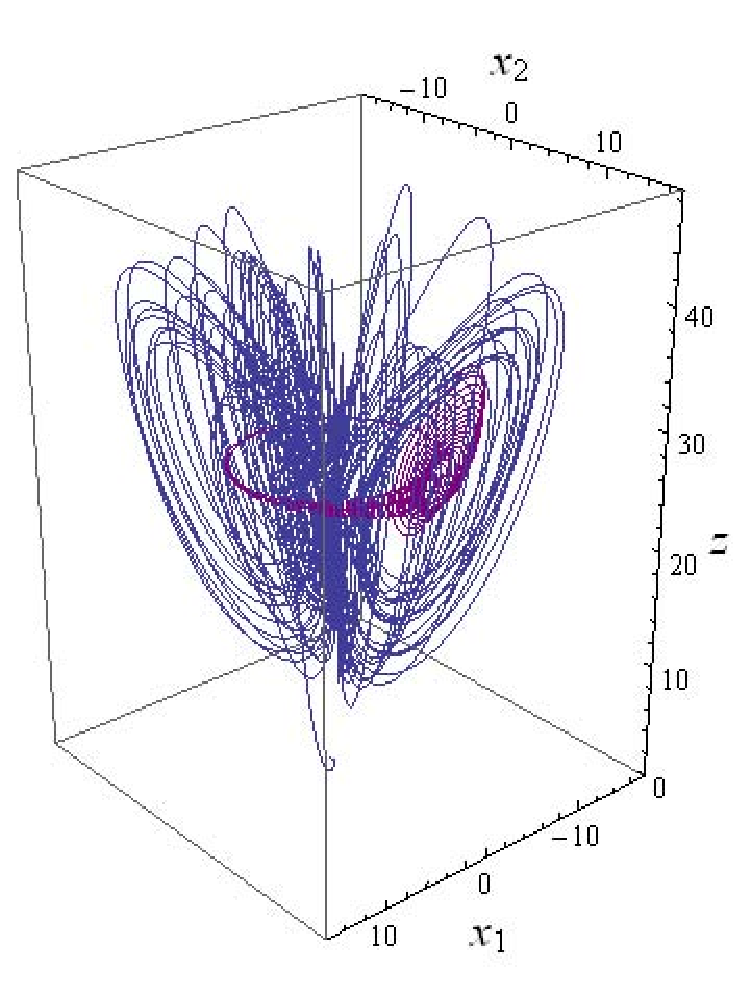
\includegraphics[width=0.35\textwidth]{CLEx1x2zRelEqu}
\end{center}
\caption{
Cartesian $\{x_1,x_2,z\}$ plot of the \cLf\ (a) with initial point
close to $\REQB{1}$, (b) superimposed over the strange attractor of
\reffig{fig:CLEx1x2z}.
    }
\label{fig:CLERelEqui}
\end{figure}
%%%%%%%%%%%%%%%%%%%%%%%%%%%%%%%%%%%%%%%%%%%%%%%%%%%%%%%

From
here on, we examine the properties of the point defined
above as $\ssp_{\REQB{}1}$.

\subsection{Eigen-system of the slice \stabmat}

As in \refsect{sect:stability}, we now find and plot the eigensystem of the \stabmat\ in order to understand the stability of $\REQB{1}$.
Rebecca finds the eigenvalues
\[
(\lambda_{1,2},\lambda_3,\lambda_4)
= (0.0938179 \pm 10.1945 i,-11.0009,-13.8534)
\]
with the eigenvectors
\bea
\Re e_{1} &=& \Re e_{2} = (-0.266121, -0.0321133, 0.00034139, 0.719222)
\continue
\Im e_{1}  &=& -\Im e_{2} = (-0.295017, 0.569063, -0.000551886,0)
\continue
e_3 &=& (-0.0883591, -0.0851485, -0.989135, -0.0809553)
\continue
e_4 &=& (-0.855586, -0.329912, -0.00273531, -0.398902)
\,.
\label{eigVecQ1}
\eea

As in \refsect{sect:stability}, we can also plot the flow
with an initial point very near to
$\REQB{1}$ along one of the eigenvectors.
% \refFig{fig:CLEQ1} shows just this.
                                                    \exerbox{exer:EigenQ1}
                                                    \exerbox{exer:PlotPolEigenQ1}

\section{\Reducedsp}
\label{sect:reducedStateSp}

Finally, we move on to the goal of the project, reducing the
state-space of the \cLe\ to only four dimensions. We present
two different versions of the `method of moving frames.' The
method can introduce singularities, as in
\reffig{fig:PCsimulPolar}.

\subsection{Method of moving frames, finite time steps}
\label{sect:MovFrame}

     \Private{
\noindent{\bf Predrag -
July 19, Aug 12 2009}: %\\
    }

Siminos\rf{SiminosThesis} discusses symmetry reduction by the
method of {\em moving frames} of Cartan\rf{CartanMF}, in the
formulation of Fels and
Olver\rf{FelsOlver98,FelsOlver99,OlverInv}.
                                                \exerbox{exer:SO2cSect}
The moving frames method allows the determination of (in
general non-polynomial) invariants of the group action by a
simple and efficient algorithm that, as argued in
\rf{SiminosThesis}, works well in high-dimensional \statesp s.

Split up the integration of the $\SOn{2}$-equivariant ODE into
a sequence of short time steps, each followed by a rotation
such that the next segment initial point is in the point
$\sspRed$ {\slice}, a $(d\!-\!1)$-dimensional hyperplane
normal to the group rotation tangent $\sliceTan{}$ at point
$\sspRed$:
\beq
(\ssp- \sspRed) \cdot \sliceTan{}=0
    \,,\qquad
\sliceTan{} = \Lg \cdot \sspRed
\,.
\ee{PCsectQ}
For any $\hat{\ssp}$, $\ssp =
\LieEl(\gSpace)\cdot\hat{\ssp}$ is defined to be the
rotation of $\hat{\ssp}$ that lies in the \slice. Such a
map from a point in space to the group action is called a
\emph{moving frame} in the formulation of Fels and
Olver\rf{FelsOlver98,FelsOlver99,OlverInv}.

[...]
                                                    \exerbox{exer:PCsectionCLe}

%%%%%%%%%%%%%%%%%%%%%%%%%%%%%%%%%%%%%%%%%%%%%%%%%%
% computed by PCunrot.nb
\SFIG{ProblemsPill} %PCunrot}
{}{
Method of moving frames, finite time steps version: a
trajectory started on the \slice, with $\ssp_1^{(0)}
=0$, evolves for a finite time to a \statesp\ point with a
non-zero $\hat{\ssp}_1^{(1)}$. The {\em entire} \statesp\ is then
rotated (the `frame is moved') so that the equivalent point
on the circle lies on the \slice, $\ssp_1^{(1)} =0$.
Thus after every finite time step followed by a rotation the
trajectory returns to the 4$\dmn$ $\ssp_1 =0$
\reducedsp.
}
{fig:PCunrot}
%%%%%%%%%%%%%%%%%%%%%%%%%%%%%%%%%%%%%%%%%%%%%%%%%%

\refFig{fig:PCunrot} illustrates the method of moving frames,
finite time version.
    \PC{Draw your own \refFig{fig:PCunrot}
        - need to draw a longer segment of the initial trajectory,
        to make it clearer that the whole segment is rotated.
       }

\subsection{Method of moving frames, differential formulation}
\label{sect:MovFrameODE}


\begin{bartlett}
I made a wrong mistake.
\bauthor{Yogi Berra}
\end{bartlett}


                                                    \exerbox{exer:CLEsmall-x1x2}
                                                    \exerbox{exer:csectionCLeODE}
                                                    \exerbox{exer:csectionPhase}
                                                    \exerbox{exer:SiminosSlice}
Infinitesimal time version of the moving frames symmetry
reduction is attained by taking small time steps in
\reffig{fig:PCunrot} and dropping the higher order terms, as
in \refsect{sect:SymmDyn}.

%%%%%%%%%%%%%%%%%%%%%%%%%%%%%%%%%%%%%%%%%%%%%%%%%%
% File: infMF.xfig
\SFIG{ProblemsPill} %infMF}
{}{
Method of moving frames, infinitesimal formulation.
}
{fig:infMF}
%%%%%%%%%%%%%%%%%%%%%%%%%%%%%%%%%%%%%%%%%%%%%%%%%%

    \PC{Draw your own \reffig{fig:infMF}.
        }
                                                        \exerbox{exer:csectionReduced}
    \PC{
A more elegant derivation is given in
\refrefs{rowley_reconstruction_2000,rowley_reduction_2003}.
    }


%
%%%%%%%%%%%%%%%%%%%%%%%%%%%%%%%%%%%%%%%%%%%%%%%%%%%%%%%%%%%%%%%%%%
% CLEpcSect.png computed by  CLEfinal.nb (repo: vaggelis)
% CLEpcSect2.png computed by CLEfinal.nb (repo: vaggelis)
\begin{figure}[ht]
\begin{center}
(a) % 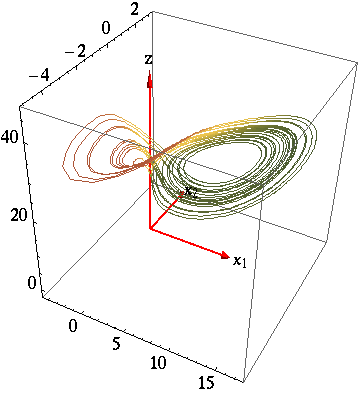
\includegraphics[width=0.40\textwidth]{CLEpcSect}
(b) %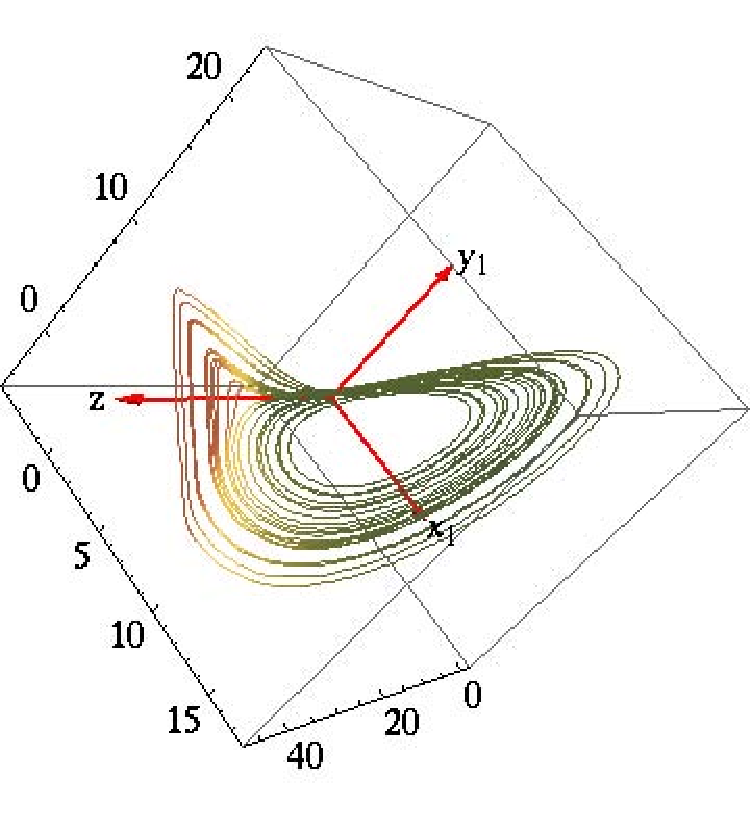
\includegraphics[width=0.43\textwidth]{CLEpcSect2}
\end{center}
\caption{
Method of moving frames, \slice\ fixed by a point on an
\reqv\ group orbit, $\sspRed = \ssp_{\REQB{}1}$. The strange
attractor of \reffig{fig:CLEx1x2z} in the \reducedsp\
of \refeq{EqMotionMovFramePC}:
(a) $\{x_1,x_2,z\}$ projection,
(b) $\{x_1,y_1,z\}$ projection.
Color-coding indicates $(\hat{\ssp} \cdot \hat{\sspRed})_4$
where $\hat{.}$ stands for unit vector, with green indicating values
of the inner product close to $1$ and brown indicating values
close to $0$.
    }
\label{fig:CLEpcSect}
\end{figure}
%%%%%%%%%%%%%%%%%%%%%%%%%%%%%%%%%%%%%%%%%%%%%%%%%%%%%%%%%%%%%%%%
%
A long time trajectory of \refeq{EqMotionMovFramePC} with
$x^*$ on the \reqv\ \REQB{1} group orbit is shown in
\reffig{fig:CLEpcSect}.
                                                        \exerbox{exer:PCsectionCLe}
    \PC{draw your own \reffig{fig:CLEpcSect}:\\
        * Mark $\ssp_{\REQB{}1}$ \\
        * Draw stable eigenvector of $\ssp_{\REQB{}1}$\\
        * State value of $\ssp_{\REQB{}1}$ somewhere
        }


%%%%%%%%%%%%%%%%%%%%%%%%%%%%%%%%%%%%%%%%%%%%%%%%%%
% computed by PCunrot.nb
\SFIG{ProblemsPill} %PCunrot1}
{}{
Method of moving frames, continuous time version, for the
$\slicep=(0,1,0,0)$,
$x_1=0,\;x_2>0$, \slice. The strange attractor of
\reffig{fig:CLEx1x2z} in the \reducedsp,
$\{x_2,y_2,z\}$ projection exhibits a discontinuity at
$x_2=0$.
}
{fig:PCunrot1}
%%%%%%%%%%%%%%%%%%%%%%%%%%%%%%%%%%%%%%%%%%%%%%%%%%

The method encounters singularities in
subsets of \statesp\rf{SiminosThesis}.
                                                    \exerbox{exer:csectionCLe}
A typical trajectory is shown in \reffig{fig:PCunrot1}.

\subsection{Integration on the \slice}

Our second method of symmetry reduction Siminos
\rf{SiminosThesis} calls {\em integration on the
\slice\ (II)}.

\section{Stability of \reqva}

\subsection{Hilbert polynomials}

The polynomials \refeq{eq:ipLaser} form a Hilbert basis for the \cLe.
\beq
\begin{split}
    u_1 &= x_1^2+x_2^2 \cont
    u_2 &= y_1^2+y_2^2 \cont
    u_3 &= x_1 y_2-x_2 y_1\cont
    u_4 &= x_1 y_1+x_2 y_2\cont
    u_5 &= z\,.
    \label{eq:ipLaser}
\end{split}
\eeq
In terms of the polar coordinates for the \cLe, these polynomials are
	\PC{shouldn't the first two be $\rho_1^2,\rho_2^2 $?}
\beq
\begin{split}
    u_1 &= \rho_1 \cont
    u_2 &= \rho_2 \cont
    u_3 &= - \rho_1 \rho_2 \sin \theta \cont
    u_4 &= \rho_1 \rho_2 \cos \theta \cont
    u_5 &= z\,.
    \label{eq:hilPolar}
\end{split}
\eeq
The \cLe\ in the Hilbert basis are:
\beq
\begin{split}
  \dot{u}_1 &=2\,\sigma\,(u_4-u_1)\,,\\
  \dot{u}_2 &=-2(\,u_2 - r_2\, u_3 -\,(r_1-u_5)\,u_4)\,,\\
  \dot{u}_3 &=-(\sigma\, +1)\,u_3+r_2\, u_1+e\, u_4\,,\\
  \dot{u}_4 &=-(\sigma\, +1)\,u_4+\,(r_1-u_5)\,u_1+\sigma\, u_2-e\,u_3\,,\\
  \dot{u}_5 &=u_4-b\, u_5\,.
\end{split}
\label{eq:CLEip}
\eeq
The {\reqv} in polar coordinates is $\left( \rho_1 , \rho_2 , \theta , z \right) = \left(\sqrt{b \left(r_1 -d\right)},\sqrt{b d \left(r_1 -d\right)},\theta_Q, r_1 -d\right)$ where $d = 1+ \frac{e^2}{(\sigma +1 )^2}$ and $\theta_Q$ is the angle such that $\cos \theta_Q = \sqrt \frac{1}{d}$ and $\sin \theta_Q = -\sqrt \frac{d-1}{d}$.

\exercise{Hilbert basis singularities}{\label{exer:CLEipSyz}
% Predrag extracted from siminos/blog/CLEflotsam      Jun  5 2010
% also ChaosBook \example{Hilbert basis singularities}{\label{exam:CLEipSyz}
%
When one takes syzygies into account in rewriting a
dynamical system, singularities are introduced. For instance,
eliminate $u_2$ using the syzygy, and show that you get
the reduced set of equations,
	\PC{I removed
$  \dot{u}_2 = -2\left(\,\frac{u_3^2+u_4^2}{u_1} - \rho_2\, u_3
                -\,(\rho_1-u_5)\,u_4\right)
$
            }
\bea
  \dot{u}_1 &=& 2\,\sigma\,(u_4-u_1)
                \continue
  \dot{u}_3 &=& -(\sigma\, +1)\,u_3+\rho_2\, u_1+e\, u_4
                \continue
  \dot{u}_4 &=& -(\sigma\, +1)\,u_4+\,(\rho_1-u_5)\,u_1
                +\sigma\, {(u_3^2+u_4^2)}/{u_1}-e\,u_3
                \continue
  \dot{u}_5 &=& u_4-b\, u_5
\,,
\label{eq:CLEipSyz}
\eea
singular as $u_1\rightarrow 0$. (PC: check this - there might
be errors)
\authorES{}
    } %end \exer{Hilbert basis singularities}

The {\stabmat} in the Hilbert basis for the \cLe\ is
	\PC{This is [5$\times$5], but there are only 4 independent
            variables. How does that show up in the eigensystem of
	    {\stabmat}?}
\beq
\begin{split}
\mathbb{A}=
\left(
\begin{array}{ccccc}
-2 \sigma & 0 & 0 & 2 \sigma & 0\\
0 & -2 & 2 r_2 & 2 (r_1 - u_5) & -2 u_4\\
r_2 & 0 & -(\sigma +1 ) & e & 0\\
(r_1 -u_5 ) & \sigma & -e & -(\sigma +1 ) & -u_1\\
0 & 0 & 0 & 1 & -b
\end{array}
\right)
\end{split}
\eeq

\subsection{Stability in \reducedsp}
%SF June 22 2010
Using the usual parameters, we get the eigenvalues $0.0938 \pm 10.1945i,-22.0000,-13.8534,-11.009$ with corresponding eigenvectors$\left(0.3378\mp 0.3411i,0.6887,0.0017\mp 0.0031i,0.5133\mp 0.1706i,-0.0029\mp 0.0511i\right),\left(0.9939,0.0470,0.0009,-0.0994,0.0051\right),\left(-0.8966,0.3457,0.0097,-0.2755,0.0246\right),\left(0.0210,-0.0203,-0.995,0.0095,-0.0011\right)$
These are the same as the eigenvalues found using polar coordinates with the addition of $-22.0000$.

The equations of motion for trajectory kept in a hyperplane by rotation under the symmetry group are:
\bea
    \dot{\gSpace}_a (y)=\frac{v(y)^T \sliceTan{a}}{t(y)^T \sliceTan{}}
    \continue
    u(y)=v(y)-\dot{\gSpace} (y) t(y)
\eea
where $v(y)$ is the velocity of the full \statesp\ flow, $t(y)$ is the tangent to the group action, and $\sliceTan{}$ is the vector normal to the hyperplane of the slice. Using this equation we get that the {\stabmat} $M$ for the system in reduced state space is given by:
\beq
M_{ij} = A_{ij}-c I_{ij} -(Tx)_i\,(\frac{\frac{\partial v}{\partial x_i}\cdot t'}{Tx \cdot t'} - c \frac{\frac{\partial (Tx)}{\partial x_j}\cdot t'}{Tx \cdot t'})
\eeq
                                                    \exerbox{exer:Reducedstab}

                                                    \section{Conclusions}

Both the {\mslices} (or the \mframes) integration within the
\slice\ are still under development.\PC{to Stefan: keep
editing this every so often}

Future work should investigate in more depth [...].
New methods [...] In this project I have discussed, understood,
and tested [...] as applied to \cLe\.
Much work still remains before these are viable
methods for higher-dimensional flows.

